\documentclass[a4paper,11pt,twoside,openright]{book} % Type du document

% compiler avec : pdflatex, bibtex, pdflatex, pdflatex


% +---------------------------------------------------------------+
% | Language
% +---------------------------------------------------------------+
\usepackage[T1]{fontenc}
\usepackage[utf8]{inputenc}
\usepackage[french]{babel}

\newif\ifisconfidential	\isconfidentialfalse

\newif\ifisdraft\isdraftfalse



% +---------------------------------------------------------------+
% | Paramètres
% +---------------------------------------------------------------+

\newcommand{\TBtitle}{Titre du TB}
\newcommand{\TBsubtitle}{Sous-titre}%laisser vide si pas de sous-titre
\newcommand{\TByear}{2020}
\newcommand{\TBacademicYears}{2019-2020}

\newcommand{\TBdpt}{Département des Technologie de l'information et de la communication (TIC)}
\newcommand{\TBfiliere}{Filière Télécommunications}
\newcommand{\TBorient}{Orientation Sécurité de l'information}

\newcommand{\TBauthor}{Gil Balsiger}
\newcommand{\TBsupervisor}{Prof. Alexandre Duc}
\newcommand{\TBindustryContact}{Nom}
\newcommand{\TBindustryName}{EntrepriseZ}
\newcommand{\TBindustryAddress}{%
  Rue XY\\
  1400 Yverdon-les-Bains
}

% Confidentiel?
% uncomment if confidential / comment if not confiential
% \isconfidentialtrue

\newcommand{\TBresumePubliable}{
Dans ce travail... Ceci est le résumé publiable...
}

% +---------------------------------------------------------------+



% +-[set path]-------------------------------------+
\usepackage{template/TB-style}
\usepackage{template/TB-macros}
\usepackage{template/TB-template}
%\graphicspath{images/}


\begin{document}

\frontmatter
\pagestyle{empty}

% TITLE and template
% +---------------------------------------------------------------+

\TBmaketitle

\pagestyle{frontmatter}

\TBsecondTitle

\TBpreambule

\TBauthentification


% Cahier des charges
% +---------------------------------------------------------------+
\chapter{Cahier des charges}



\section*{Résumé du problème}

Le Bitcoin est la cryptomonnaie la plus connue et une des plus utilisées aujourd'hui en 2021. Cependant, elle n'est pas parfaite et certains points sur son fonctionnement et sa conception peuvent poser problème. Le premier est que la vérification des transactions est très consommatrice d'énergie. A titre d'exemple, la puissance totale de tous les mineurs de Bitcoin regroupés permettrait d'alimenter un pays de taille comparable aux Pays-Bas\cite{BTC_cons}. Le deuxième problème est que les transactions sont consultables publiquement ce qui pose un problème de confidentialité. Il est possible de voir le montant de chaque transaction et ainsi remonter la blockchain pour trouver le solde d'un compte. Cela n'est pas adapter à des transactions plus sensibles comme des versements de salaire par exemple.

\subsection*{Problématique}

En prenant en compte les deux problèmes majeurs du Bitcoin décrits ci-dessus, on peut en déduire que le Bitcoin n'est plus dans l'air du temps même si il est encore très populaire. La problématique est la suivante: il faut trouver une alternative écologique et confidentielle au Bitcoin.

\subsection*{Solutions existantes}

Aujourd'hui en 2021, il existe une multitude de blockchains et cryptomonnaies. Cependant la majorité d'entre elles utilisent le même principe énergivore que Bitcoin ou sont des tokens sur la blockchain Ethereum qui n'est, en 2021, ni plus écologique ni plus confidentielle que Bitcoin.

Mais il y a tout de même des solutions existantes. Il existe des algorithmes beaucoup moins énergivores que la vérification par preuve de travail (Proof-of-Work) utilisé par Bitcoin comme Proof-of-Stake ou encore Proof-of-Space. Concernant la confidentialité, il existes des blockchains confidentielles comme Monero ou Zcash. Cependant, il n'y a pas cryptomonnaie/blockchain qui utilise un algorithme écologie et confidentielle à la fois.

\subsection*{Solutions possibles}

Une solution possible pour résoudre cette problématique est de développer une blockchain qui utilisera un algorithme écologique pour vérifier les transactions comme du Proof-of-Stake ou du Proof-of-Space. Pour les raisons de confidentialité précédemment évoquées, les transactions devront être chiffrées au sein de la blockchain pour pas que leurs montants ou les adresses ne soient consultables publiquement.

\section*{Cahier des charges}

\subsection*{Objectifs}

\subsection*{Besoins}

\subsection*{Contraintes}

\subsection*{Déroulement}

\subsection*{Livrables}
Les délivrables seront les suivants :
\begin{enumerate}
\item Une documentation contenant :
	\begin{itemize}
	\item Une analyse de marché
	\item La décision qui découle de l’analyse
	\item Spécifications
	\item Les informations du module tel que le fonctionnement et les limitations 
	\item Une planification initiale et finale
	\item Un mode d’emploi
	\end{itemize}
\item Un module remplissant les objectifs défini au point 2.1.
\item Un software implémentant les améliorations s’il a été possible de les effectuer.
\end{enumerate}



% TOC
% +---------------------------------------------------------------+
\tableofcontents
\clearpage


% Content
% +---------------------------------------------------------------+

\mainmatter
\pagestyle{plain}

\chapter{Introduction}
\label{ch:intro}


%exemple
\lipsum[1-4]



\chapter{État de l'art}
\label{ch:etatdelart}


%exemple
\lipsum[1-4]


\chapter{Exemple de chapitre}

\lipsum[1]


\section{images ?}

Voici comment mettre une image.

\begin{figure}
	\centering
	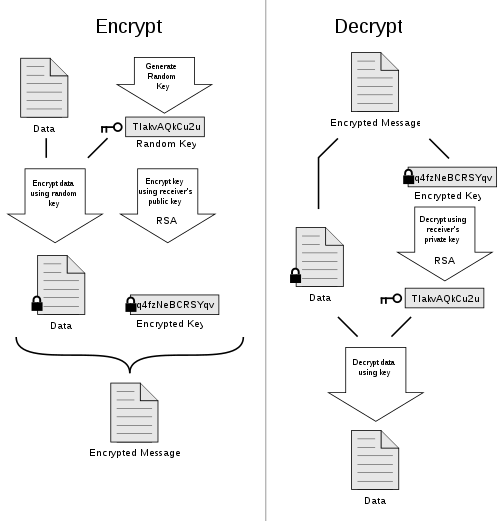
\includegraphics[width=8cm]{images/PGP_101.png}
	\caption{Schéma PGP}
	\label{fig:pgp}
\end{figure}


\section{comment citer une référence bibliographique ?}

Ceci est un exemple de citation d'un livre de Pasini~\cite{pasini2015}.

Mais aussi du site Web de Black Alps 2019~\cite{BA19} !


\section{comment faire une référence ?}

On peut aussi ajouter une référence à la section~\ref{sec:shell}.

On peut aussi ajouter une référence à l'introduction, chapitre~\ref{ch:intro}.

Comme montre la Figure~\ref{fig:pgp}, on peut référencer une figure.


\section{comment afficher une commande simple ou du bash}

Utiliser la commande \com{com}.

Exemple : Test d'une commande bash shell \com{ls} : 

Utiliser l'environnement \com{shellcmd}.

\begin{shellcmd}
$> ls -al test_underscore $$* "coucou"
\end{shellcmd}
Bli bLa


\section{Commande Shell}
\label{sec:shell}

Voici comment faire une mise en forme de commande SHELL.

Utiliser l'environnement \com{listingsbox}.
\begin{description}
 \item[1er paramètre:] le ype de shell, ici "console"
 \item[2ème paramètre:] le nom à donner à la box
\end{description}

\begin{listingsbox}{console}{Exemple de commande shell avec réponse}
root@kali:~$ bunzip2 data-decrypted.bin
bunzip2: Can't guess original name for data-decrypted.bin -- using
data-decrypted.bin.out
\end{listingsbox}


\section{Code inclus en direct dans le latex}

Utiliser l'environnement \com{sourcebox}.
\begin{description}
 \item[1er paramètre:] le ype de shell, ici "c"
 \item[2ème paramètre:] le nom à donner à la box
\end{description}

\begin{sourcebox}{c}{Exemple de code C}
#include <stdio.h>

int main(int argc, char* argv[])
{
   printf("Hello World!\n");
   return 0;
}
\end{sourcebox}



\section{Code à partir d'un fichier}

Utiliser la commande \com{inputsourcecode}.
\begin{description}
 \item[1er paramètre:] le ype de shell, ici "c"
 \item[2ème paramètre:] le nom du fichier source, "\path{source_code/example.c}"\\ Egalement exemple de la commande \com{path}.
 \item[3ème paramètre:] le nom à donner à la box
\end{description}


%% Inclure du code source d'un fichier externe
%% 1er paramètre: langage du code
%% 2ème paramètre: le path du fichier source
%% 3ème paramètre: le titre de la box
\inputsourcecode{c}{"source_code/example.c"}{example.c}

Même exemple, mais en spécifiant les lignes 4 à 8 :
\inputsourcecode[firstline=4,lastline=8]{c}{"source_code/example.c"}{example.c}





\chapter{Architecture}
\label{ch:arch}


%exemple
\lipsum[1-4]



\chapter{Implementation}
\label{ch:impl}


%exemple
\lipsum[1-4]



\chapter{Conclusion}

\section{Résultat final}

Ce travail a mis l'accent tout particulièrement sur l'analyse des protocoles de consensus et l'implémentation du \emph{proof of space}. Et c'est dans un deuxième temps, après avoir réalisé une implémentation fonctionnelle du proof of space que la création d'une blockchain a été entreprise. La blockchain développée avait pour objectif de donner un exemple d'utilisation du proof of space avec un cas concret. De plus, sa confection m'a permis d'en savoir plus sur le fonctionnement des cryptomonnaies.

Concernant les protocoles de consensus, il y en a beaucoup qui sont intéressants mais nouveaux et donc n'ont pas énormément été utilisé concrètement. Côté écologie, le proof of work est le pire loin devant les autres mais reste avec la preuve de sécurité la plus fiable. Mais le soucis écologique qu'il pose tend les blockchains à migrer vers d'autres protocoles plus efficaces et consommant moins d'énergie. Le proof of space est un protocole tout à fait intéressant qui a suscité pas mal d'intérêt. C'est pourquoi il été choisi pour être implémenté. Le proof of stake est peut-être le deuxième protocole le plus populaire après le proof of work, il est cependant plus difficile à mettre en place sur une nouvelle cryptomonnaie puisque qu'il faut justement miser une partie de cette monnaie. Il reste quand même un bon protocole écologique.

Il est difficile de faire un classement des protocoles étudiés mais on peut dire que proof of space et proof of stake sont deux protocoles répondant aux problèmes écologiques dû au faible besoin de puissance de calcul. Proof of authority sera plus adapté pour des blockchains privées puisqu'il est plus facile de mettre en place des validateurs de confiance dans le secteur privé. Proof of history n'est certes pas un protocole de consensus, il peut s'intégré à un protocole pour permettre un synchronisation rapide comme proof of stake avec la blockchain Solana.

Étant donnée l'importance placée sur le proof of space, c'est concernant ce dernier qu'il y a le plus de résultats. Notamment au niveau des performances où plusieurs tests de benchmark on été réalisé. La conclusion de l'implémentation est qu'il est possible de créer un plot dans le but de trouver des preuves pour un challenge donné. La construction est basée sur la phase 1 du protocole de Chia \cite{chia:construction} et a été finalement entièrement implémentée (la phase 1 pas les autres). La génération du plot final se fait en temps exponentiel par rapport à une constante $k$ alors que la vérification de preuves est très efficace et réalisable en temps constant.

\section{Difficultés rencontrées}

La majeur partie des difficultés rencontrées concerne l'implémentation du proof of space. C'était une construction assez difficile à comprendre au début et il a fallu du temps pour pouvoir l'implémenter. Il a fallu apprendre à utiliser des librairies pour manipuler des bits, ce dont on a pas forcément l'habitude. On travaille le plus souvent en octet. Il a fallu trouver un moyen d'améliorer les performances avec \emph{Rayon}, une librairie de multithreading, pour obtenir un temps d'exécution convenable. Et enfin il a fallu réaliser un moyen de trier les données sur le disque. Parce que comme le protocole génère beaucoup de données, tout ne peut pas être conservé en mémoire, il faut les stocker sur le disque dur. Après la génération, les tables doivent être triées avant de pouvoir générer la suivante. Comme ces tables peuvent atteindre plusieurs giga-octets, il a fallu développer un algorithme de tri externe. C'était une des partie les plus compliquées à faire.

Mais dans l'ensemble il n'y a pas eu de difficulté trop importante qui ait pu bloquer l'avancée du projet. Il a fallu apprendre et comprendre rapidement et il a fallu écrire pas mal de code.


\section{Objectifs non-réalisés}

Mise à part tout le travail réalisé sur le proof of space et la blockchain, il y a quand même des objectifs qui n'ont pas été atteint. Notamment le souhait de créer une cryptomonnaie confidentielle. Cet aspect précis n'as pas été réalisé par manque de temps, l'implémentation du proof of space ayant pris bien 60\% du travail. Il aurait fallu analyser les blockchains \emph{Monero} et \emph{Zcash} pour connaître quelles méthodes étaient utilisées pour sécuriser les transactions et voir s'il est possible d'en ajouter une à notre blockchain. Malheureusement cette partie du travail n'a pas pu être faite.

\section{Améliorations possibles du projet}

Il y a une infinité d'améliorations possibles pour le projet mais voici une petite liste non-exhaustive d'améliorations :

\begin{itemize}
  \item Rendre les transactions confidentielles (comme Zcash ou Monero)
  \item Implémenter les phases suivantes du proof of space (nettoyage et compression)
  \item Ajouter un moyen d'avoir un consensus sécurisé (avec des VDF par exemple)
\end{itemize}

\section{Conclusion personnelle}

Venant d'une proposition personnelle, ce travail était très important pour moi et je suis content d'avoir pu le faire comme travail de Bachelor. Il m'a permis d'en apprendre beaucoup plus sur les cryptomonnaies sur le côté technique, ce que je souhaitais initialement en proposant ce sujet. Il m'a aussi permis de découvrir des protocoles de consensus particuliers notamment le proof of space dont j'ai particulièrement apprécier implémenter la construction. J'aurai évidemment souhaiter avoir plus de temps pour pouvoir améliorer ma blockchain, peut-être faire la partie mise en réseau ou bien la confidentialité des transactions mais je suis déjà très content d'avoir pu délivrer une blockchain fonctionnelle intégrant un protocole de proof of space.

% +---------------------------------------------------------------+
\cleardoublepage
\addcontentsline{toc}{chapter}{Bibliographie}
\bibliographystyle{plain}
\bibliography{chapters/biblio}
\nocite{*} %ajoute tout ce qu'il y a dans le bibtex

\listoffigures
\listoftables

% Annexes
% +---------------------------------------------------------------+
\appendix

\chapter{Outils utilisés pour la compilation}

%exemple
\lipsum[5-6]


\chapter{Journal de travail}

\bgroup
\def\arraystretch{1.5}
\begin{longtable}[c]{l l l p{8.2cm}}
    \caption{Journal de travail}\\

    \hline
    \textbf{Semaine} & \textbf{Date} & \textbf{Temps [h]} & \textbf{Tâche}\\
    \hline
    \hline
    \endfirsthead
    
    \hline
    \textbf{Semaine} & \textbf{Date} & \textbf{Temps [h]} & \textbf{Tâche}\\
    \hline
    \hline
    \endhead
    
    \multicolumn{4}{r}{\small \it Le journal de travail continue à la page suivante.} \\
    \normalsize
    \endfoot
    
    \hline
    \endlastfoot
	
	% Semaine 1
	1
	& 26.02.2021
	& 0.5
	& Meeting avec Alexandre Duc pour lancer le projet \\
	
	\hline
	
	% Semaine 2
	\multirow{8}{*}{2}
	& 01.03.2021
	& 1
	& Recherche sur les protocoles de consensus \\
	
	& 01.02.2021
	& 1
	& Recherche sur les protocoles de Zcash \\
	
	& 02.02.2021
	& 2
	& Lecture des specs de Diem \\
	
	& 02.02.2021
	& 1
	& Recherche de librairies Rust \\
	
	& 03.02.2021
	& 2
	& Création des dépôts sur GitHub et structure de la spécification en Markdown \\
	
	& 05.03.2021
	& 0.5
	& Meeting hebdomadaire avec Alexandre Duc \\
	
	& 05.03.2021
	& 2
	& Recherche sur le protocole Proof-of-Space \\
	
	& 05.03.2021
	& 1
	& Lecture du chap. 17 du Rust book \\
	
	\hline
	
	% Semaine 3
	\multirow{1}{*}{3}
	& 08.03.2021
	& 2
	& Rédaction du cahier des charges dans le rapport \\
	
	& 09.03.2021
	& 2
	& Rédaction du rapport et journal de travail \\
	
\end{longtable}
\egroup


\end{document}
